\subsubsection{Deadlift}

A deadlift is the final exercise performed at a powerlifting competition. In this movement, the barbell starts stationary on the ground. The barbell is gripped in the hands of the lifter, and the lifter must successfully ‘stand up’ whilst holding the weight. A lift is considered complete when the lifter is in a fully upright position, with knees locked and shoulders back. This movement requires activation of the entire posterior chain, that is the use of the muscles on the rear of the legs and back. Figure~\ref{fig:dead_stages} shows an example of a deadlift.

\begin{figure}[H]
    \centering
    \subfigure[Begin]{
            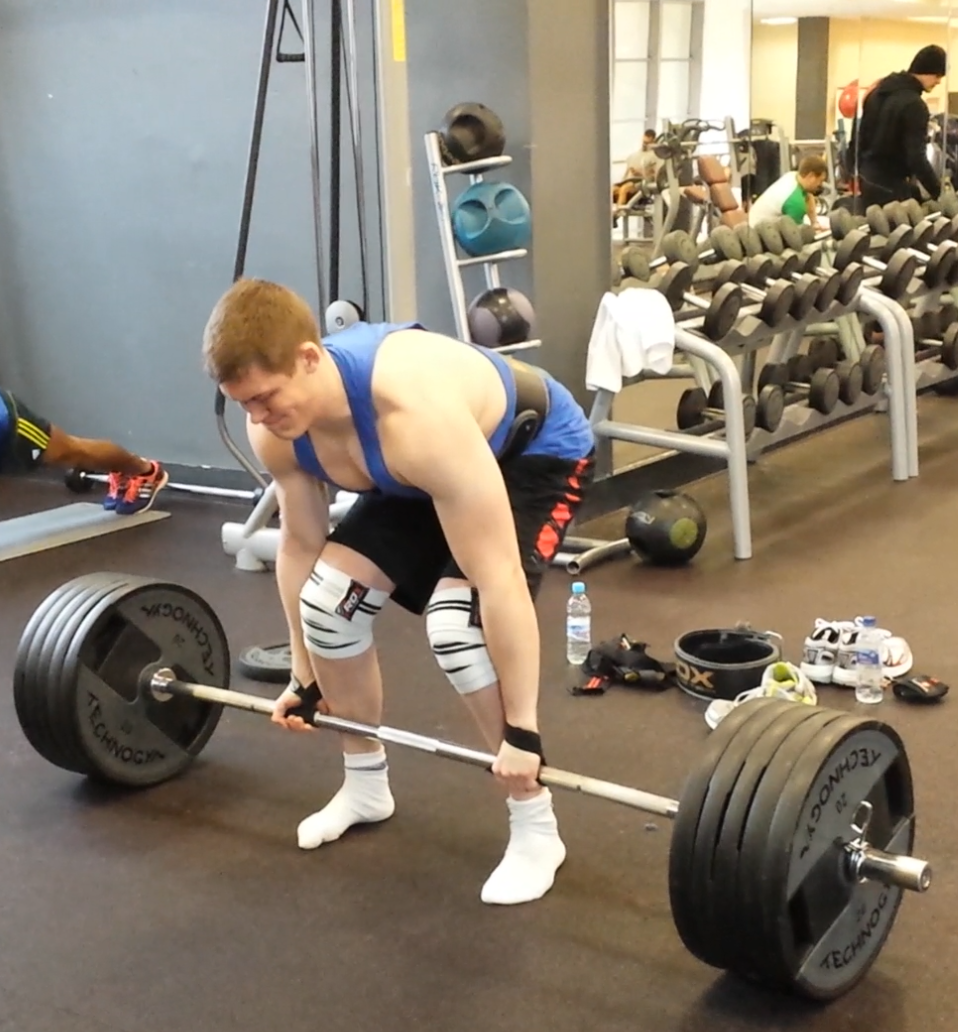
\includegraphics[height= 7cm]{intro/images/dead_bottom}
    }
    \subfigure[End]{
            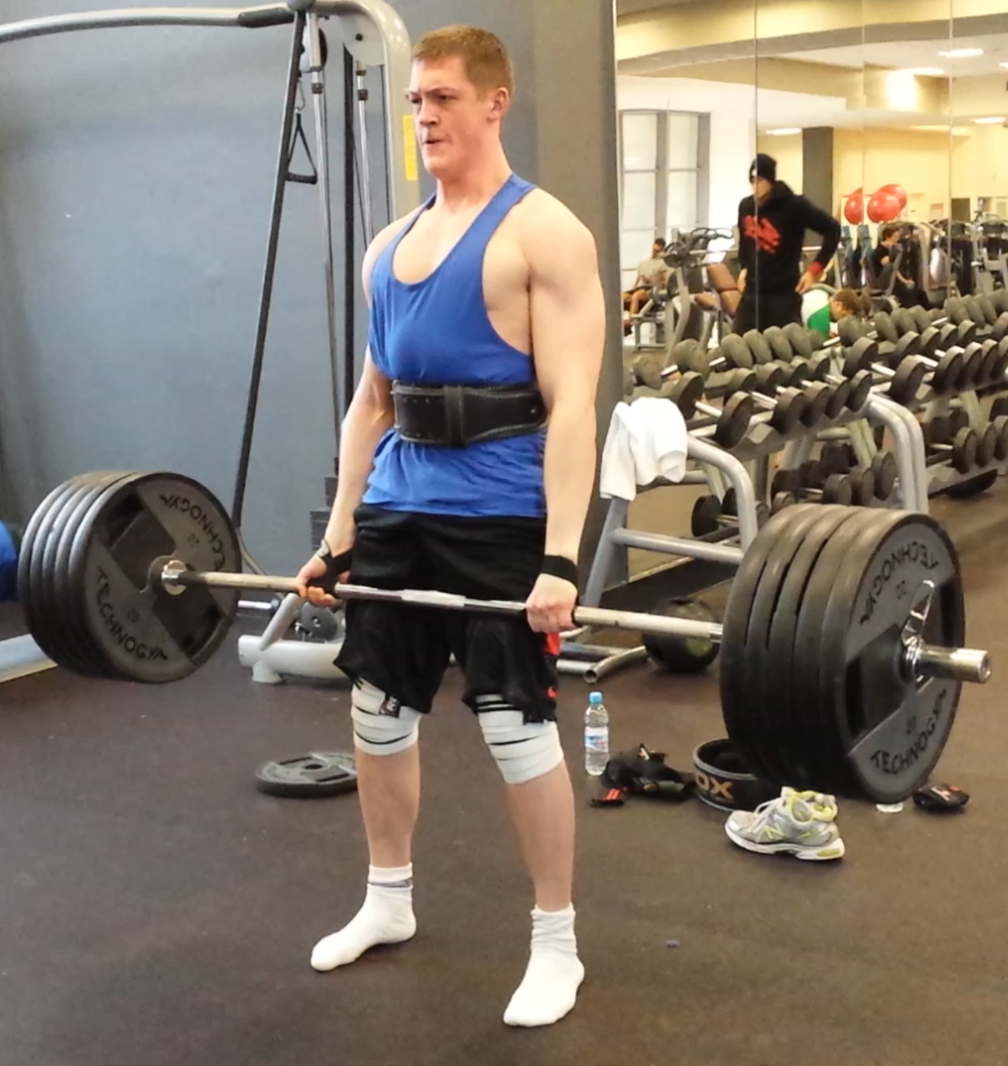
\includegraphics[height= 7cm]{intro/images/dead_top}
    }
\caption{The stages of a deadlift}
\label{fig:dead_stages}
\end{figure}

The International Powerlifting Federation regulations\cite{ipf} state that a deadlift should finish in the upright position, with no downward movement until this point. In training it is considered good practice to ensure that a neutral spine is maintained throughout the lift, that is that there should be no rounding of the back.